\section{User interface} % (fold)
\label{sec:user_interface}
This section describes in details the second part of the project.
First, an explanation will be made on the main design used in order
to have efficient command interpretation and execution.
Then will be described the effective implemenation
of the \emph{command line} user interface and the \emph{graphical} user inteface.

\subsection{Separing interpretor from processor} % (fold)
\label{sub:separing_command_getter_and_command_processor}

Thinking about the design, we quickly found a need to separate
the \emph{request} (ie. the given command) from its actual \emph{execution}.
This idea follows the open/close principle and has similar advantages
as design patterns.
It indeed allows to easily change the behaviour of the program if
one wants to change the syntax of the commands (\emph{request} class)
or what a particular command does (\emph{execution} class).
This lead to the implementation of the \CommandLine~and
the \CommandProcessor~classes.

In order to make use of commands in an efficient way,
a \Command~class is designed.
It consists of a name, a number of arguments and an array
of strings containing its arguments.
This allows the interpretor and processor to easily
communicate between themselves and with the real user.
The reader is advised to have a look at figure~\ref{fig:clui_uml}
containing the UML diagram of the relationship between
the three listed above classes.
One will notice the use of the Singleton pattern for
the \CommandProcessor~and \CommandLine.
This is justified by the fact that only one
of each will be required at the same time
and it does not created problems with \textsc{JUnit} tests
as those are made using concrete scenarios
generated by \texttt{.txt} files of commands.

\subsubsection{The \texttt{CommandLine} class} % (fold)
\label{ssub:the_commandline_class}
The \CommandLine~can be seen as the \emph{interpreter}. It will be the link
class between the real user and the system. It can either interpret commands
given directly as input with the \lstinline|launchFromInput()| method,
or listed in a \texttt{.txt} file with the \lstinline|launchFromFile| method.
Once a String that should represent a command is given to those methods,
they will call the \lstinline|getInputInfoAndProcessCmd| method whose
role is to check if the input
\begin{enumerate}
  \item corresponds to an existing command,
  \item has the ``$<>$'' argument declaration,
  \item has the right number of arguments associated with this command. 
\end{enumerate}
If one of those conditions is not satisfied, a message containing the
error description will be send back to the \lstinline|launch| method
which will print it.
On the other hand, if the conditions are satisfied, the method
creates a new \Command~object and pass it to the \lstinline|processCmd|
method of its \CommandProcessor~attribute.
% subsubsection the_commandline_class (end)

\subsubsection{The \texttt{CommandProcessor} class} % (fold)
\label{ssub:the_commandprocessor_class}
The \CommandProcessor~can be seen as the \emph{executor}.

% subsubsection the_commandprocessor_class (end)

  
%%%%%%%%%%%%%%%%% SINGLETON WITH COMMANDLINE %%%%%%%%%%%%%%%%%
% \begin{lstlisting}[caption=Singleton pattern with CommandLine class.,
%    label=lst:commandline] 
% private CommandLine() {
%   cmd_processor = CommandProcessor.getInstance();
%   command_list = ParseCommands.parseCommands("src/txtFILES/mf_commands.txt");
%   for(Command cmd : command_list) {
%     command_hm.put(cmd.getName(), cmd.getNb_args());
%   }
% }
% private static class CommandLineHolder {
%   private static final CommandLine INSTANCE = new CommandLine();
% }
% public static CommandLine getInstance() {
%   return CommandLineHolder.INSTANCE;
% }
% \end{lstlisting}


% subsection separing_command_getter_and_command_processor (end)

\subsection{Command line interface} % (fold)
\label{sub:command_line_interface}

Firstly, a note has to be made on the general choice of implementation
of the command line interface.
Following \textsc{Unix} command line style, one should be able to run
a command with multiple arguments in the following
style \lstinline|command -arg1_type arg1 -arg2_type arg2|.
In the \MyFoodora case, it seems more adequate to have one syntax for each
command, being \lstinline|command <arg1, arg2>|, which is proposed in 
the project requirements. The program will thus be able to give informations
on the commands when needed and we expect the user to quickly remember 
the commands, as there is only few of them for each user type.
 
The choice of implementation described in the first paragraph
lead us to the use of an \lstinline|HashMap<String, Integer>| to
store the list of commands and their associated number of arguments,
as we only have \emph{one} number of arguments for one command.

Once we had the general design of the user interface, we began to
think there might be a design pattern which used \Command, \CommandLine~and
\CommandProcessor~classes.
We discovered the \emph{command design pattern}~\cite{wiki:commandPattern},
which lead us to some improvements of the code.

In terms of effeciency, using a parallel \lstinline|HashMap| to store
the commands names and their associated number of needed arguments,
allows to check if the given command name exists in $\mathcal{O}(1)$
time on average and in $\mathcal{O}(\log{n})$ on worst case
(this happens when collisions happen, ie. the \lstinline|HashMap|
entries container is not big enough)\cite{hashMap}.

see fig.~\ref{fig:clui_uml}

\begin{figure}
  \begin{center}
    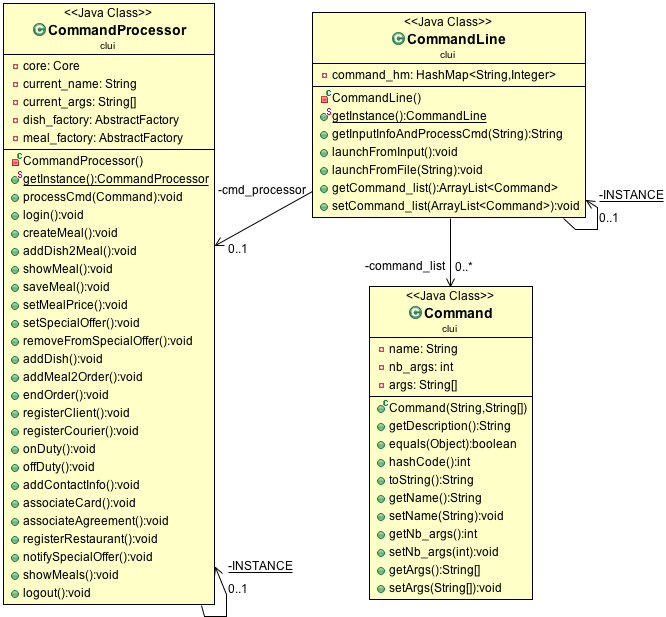
\includegraphics[scale=0.5]{./img/CLUI.png}
    \end{center}
  \caption{\umld of the command line user interface.}
  \label{fig:clui_uml}
\end{figure}

% subsection command_line_interface (end)

\subsection{Graphical interface} % (fold)
\label{sub:graphical_interface}

% subsection graphical_interface (end)
% section user_interface (end)